%\documentclass[11pt,a4paper,oneside]{report}

%\usepackage{tikz}
%\usetikzlibrary{arrows,automata}
%\usepackage{float}
%\usepackage{caption}
%\usepackage{changepage}

%\begin{document}

%----------------------------------------------------------------------------
\chapter{Runtime Architecture}\label{sect:RuntimeArch}
%----------------------------------------------------------------------------

Running games require the execution of untrusted code --- in form of both the game engine and the bots --- in a safe manner, which is complex task.

The limitations of java's security error handling make the jvm unable to provide a platform where a whole game --- all of the actors and client runtimes --- can be run as a single process. Therefore separate java processes are necessary to achieve a safe runtime environment. 

	\section{Runtime model}
	
	The runtime model consists of two main types of entities: the runtime handler that acts as the controller of a played game, and actor client runtimes that manage the individual actor participants.   
	They communicate with each other over standard TCP sockets organized into a star topology with the handler at its center.
	
	\section{Runtime handler}
	
	The runtime handler is the central managing entity of a given game, it initiates most operations through controlling the client runtimes, and processes their responses. Its job is mainly to:
	
	\begin{itemize}
		\item Provide the necessary binaries to the client runtimes, including the game api, engine, or bot libraries.
	
		\item Control the game flow based on a general ask--answer turn based system.
		
		\item Process log messages from the actors.
	
		\item Process error reports from the actor runtimes.
		
		\item Report the result of the game, whether the engine reported a 'normal' finish or some error occurred.  
	\end{itemize}
	
	The handler is a library which can be used from other jvm-based programs, as it exposes functions to run games using provided actors.
	
	\section{Actor client runtimes}
	
	Actor client runtimes are executable java processes that are responsible for communicating with the runtime handler, providing a secure environment in which the given actor can be used, processing requests from the runtime handler, driving the actors in response to the received control messages, and reporting any problems that might occur during the game.
	They come in two forms, based on whether they manage a game engine or a bot, as the two tasks require different messages and control structure.

	 The runtimes are isolated programs, that only need to know the way of connecting to the handler to run, as they actually receive the actor to be managed and other libraries through standard messages after startup. This allows a flexible separation of the runtimes as long as a connection can be provided between them. If, for example, extra security or scalability is warranted, the design would allow running these clients on different physical- or virtual machines, or other containers.
	
	All actor client runtimes provide logging facilities to their respective actors, which can be used to save messages to be viewed by the creator of the actor after the game has ended.
	
	Beside direct client-handler messaging --- such as logging or error reporting ---, the runtime model also needs to manage inter-actor communication to allow an engine to interact with the bots. This is manifested as one directional method calls as --- due to the logic of the system --- only the engines have access to their bots and not in reverse.
	As these calls should happen between objects running on different java virtual machines, remote method invocation is necessary.
	
		\subsection*{Engine client runtime}
	
		On top of the client runtimes' common tasks, an engine client runtime must also provide game bot proxies to the engine it manages. Through these stubs can the environment then convert the specific call requests to standard messages, which can in turn be understood, and routed by the runtime handler. After such call is successfully evaluated by the desired bot, the response is processed by the proxy and returned transparently to the engine.
	
		\subsection*{Bot client runtime}
		
		As an engine runtime handles the stub side of the actor-bot remote communication, a bot runtime must provide a way of processing incoming invocation requests, and forward them to the bot it drives. After the target method has been executed, and some kind of result produced, it is this skeleton's task to send the outcome back through the runtime handler.

	\section{Communication model}

		Communication between the various components of the runtime model are driven by discrete messages, whose content and sequence follow a well-defined protocol enforced by the runtime handler and clients. These messages either provide standalone information, or form a more complex transaction. Any message that breaks the expected flow of communication will trigger errors in the clients, but it is usually the handler that interrupts the game, should any discrepancy occur.
		
		Some messages can be closely tied to actor operations, while others help to operate the runtime model. 

		Messages carry three types of information: their type, the type's optional parameters, and an optional payload as well. The type is to determine the objective of the message, while the type parameters and payload are to carry variable information of the instance of the message. The latter two's separation is an implementational decision that ensures safe message handling. As such, from the communication model's perspective, they can be viewed as a combined payload, and in the remainder of this chapter will be referred to as 'payload' or 'data'.  

		\subsection*{Simple messages}
		
		Simple messages carry pieces of information that are meaningful on their own, either from an actor client to the handler or in the opposite direction. They do not represent an answer for another message, and no such answer is expected to be replied to them.
		
		\begin{figure}[H]
			\centering
			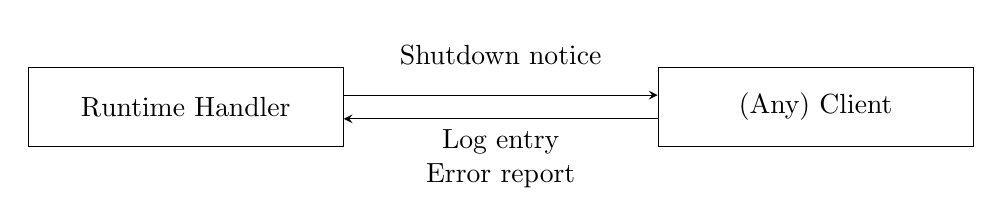
\begin{tikzpicture}[->, >=stealth, rectangle, every node/.style={minimum height=1cm, minimum width=4cm}, node distance=8cm, auto]
			
				\node [draw] (H) {Runtime Handler};
				\node [draw] (C) [right of = H] {(Any) Client};

				\draw [transform canvas={yshift=0.15cm}] (H) edge node[above, align=center]
				{Shutdown notice} (C);
				
				\draw [transform canvas={yshift=-0.15cm}] (C) edge node[below, align=center]
				{Log entry\\Error report} (H);
				
			\end{tikzpicture}
			\caption*{\emph{Possible simple messages between handler and bot- or engine client}}
		\end{figure}
		
		\begin{figure}[H]
			\centering
			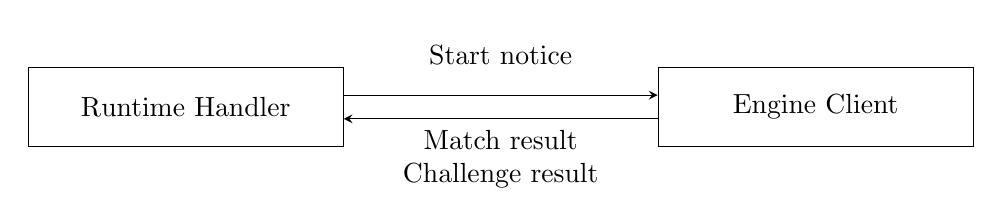
\begin{tikzpicture}[->, >=stealth, rectangle, every node/.style={minimum height=1cm, minimum width=4cm}, node distance=8cm, auto]
			
				\node [draw] (H) {Runtime Handler};
				\node [draw] (EC) [right of = H] {Engine Client};

				\draw [transform canvas={yshift=0.15cm}] (H) edge node[above, align=center]
				{Start notice} (EC);
				
				\draw [transform canvas={yshift=-0.15cm}] (EC) edge node[below, align=center]
				{Match result\\Challenge result} (H);
				
			\end{tikzpicture}
			\caption*{\emph{Possible simple messages between handler and engine client}}
		\end{figure}
		
			\paragraph{Start notice}
			
			This message is only sent once per game to the engine client, as a signal that all actor clients have received all the data (api and actor binaries) that they needed to start working, and a game may be started. Following its reception the engine client starts the game by invoking the engine object's \code{playGame} method.
		
			\paragraph{Shutdown notice}
			
			This message can be sent at any time during the game, and signals its end --- either due to some error happening or normal game completion --- to the clients, who after receiving it should finish all running tasks, and stop themselves.
		
			\paragraph{Log entry}
			
			Log messages are the only non-control messages, due to them not affecting the flow of the game in any way. They carry their target (the actor or actors whose log will contain the message) and their message itself as their payload. They are sent at any time by one of the actor clients, and are processed independently of the control messages by the runtime handler.
			
			\paragraph{Error report}
			
			Much like log entries, error reports can be sent at any time; however, instead of being actor initiated, they are generated by the client runtime if any irregularity has happened. They can be caused by execptions thrown in the actors' code, unexpected runtime behavior, or attempted access to guarded resources by the actor. As they signal unrecoverable errors, the runtime handler will interrupt the game after receiving them, and choose a result fitting the context the report was created in and the information it carries.
			Based on these pieces of information, the handler will generally mark the game as ended with:
			
			\begin{itemize}
				\item An error caused defeat of the bot of the report's sender (e.g. in case of attempted permission violation or general exception in the bot's code).
				
				\item An error (no winner or loser) if the error occurred not in the actor's, but in the runtime's code
				
				\item Game error if the report was sent from the engine's client due to the former's failure. 
			\end{itemize}
			
			\paragraph{Match result, Challenge result}
			
			Signals from the engine client that imply the engine object's \code{playGame} method successfully finished. They carry the data containing the game's result in accordance with the game model's description. If no error has happened, they act as the signal for the end of the game, and as such may be viewed to form a non-simple message pair with start notice.
			
		\subsection*{Actor binary transfer}
		
		Actor binary messages serve as both parts of a request--response pair. When making a request, a client asks the handler for a type of binary resource required to do its job --- the game's api, engine, or the managed bot. The handler in return sends back the requested binary, while also keeping track of all such requests. If all needed binaries have been sent to all clients, the handler will initialize the start of the game using a start notice message. 
		
		\begin{figure}[H]
			\centering
			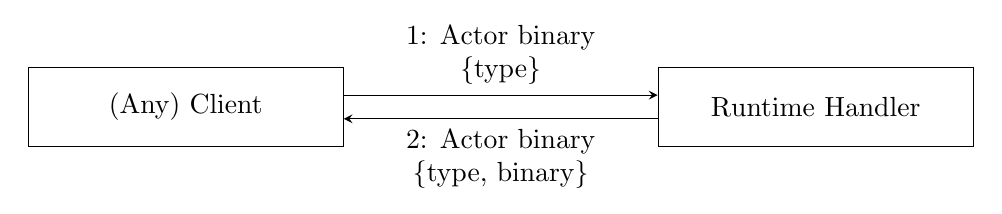
\begin{tikzpicture}[->, >=stealth, rectangle, every node/.style={minimum height=1cm, minimum width=4cm}, node distance=8cm, auto]
			
				\node [draw] (C) {(Any) Client};
				\node [draw] (H) [right of = C] {Runtime Handler};

				\draw [transform canvas={yshift=0.15cm}] (C) edge node[above, align=center]
				{1: Actor binary\\\{type\}} (H);
				
				\draw [transform canvas={yshift=-0.15cm}] (H) edge node[below, align=center]
				{2: Actor binary\\ \{type, binary\} } (C);
				
			\end{tikzpicture}
			\caption*{\emph{Actor binary request--response}}
		\end{figure}
		
		\subsection*{Remote invocation}

		Remote invocation is the most complex communication operation as it involves routing by the handler, and multiple possible valid return types.
		
		As the engine runtime's proxy captures a method call attempt by the engine object, the client sends a proxy call message containing the target bot, requested method identifier, and optional method parameters. This message is forwarded by the handler to the target client, who executes its bot's appropriate method. If this method produces a valid result under the configurable time limit, that value is returned wrapped into a call result message, all the way to the engine. If some error happens during the evaluation, (as usual) an error report is returned to the handler.
		
		However, a special case is also possible, if the bot's method does not finish in time. If this happens, instead of an error report, a bot timeout message is sent back to the engine. This bot timeout acts as a 'recoverable error' --- an event when the engine can choose to ignore the bot's shortcoming. If the engine was created without support for these occurrences, the default error processing takes place.
		
		\begin{adjustwidth}{-0.8cm}{}
		\begin{minipage}[t]{.45\textwidth}
			\begin{figure}[H]
				\centering
				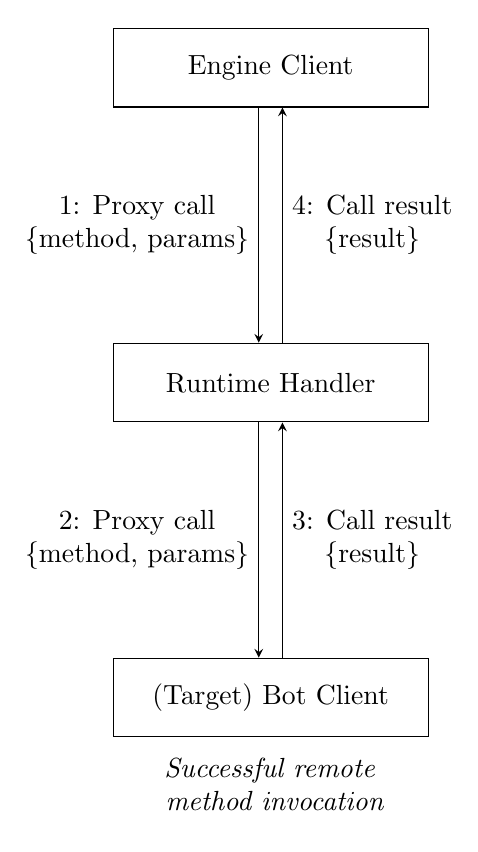
\begin{tikzpicture}[->, >=stealth, rectangle, every node/.style={minimum height=1cm, minimum width=4cm}, node distance=8cm, auto]
			
					\node [draw] (E) {Engine Client};
					\node [draw] (H) [below of = E, node distance=4cm] {Runtime Handler};
					\node [draw] (B) [below of = H, node distance=4cm] {(Target) Bot Client};

					\draw [transform canvas={xshift=-0.15cm}] (E) edge
					node[left, align=center, minimum width=0cm]
					{1: Proxy call \\ \{method, params\}} (H);
				
					\draw [transform canvas={xshift=0.15cm}] (H) edge
					node[right, align=center, minimum width=0cm]
					{4: Call result \\ \{result\}} (E);
				
					\draw [transform canvas={xshift=-0.15cm}] (H) edge
					node[left, align=center, minimum width=0cm]
					{2: Proxy call \\ \{method, params\}} (B);
				
					\draw [transform canvas={xshift=0.15cm}] (B) edge
					node[right, align=center, minimum width=0cm]
					{3: Call result \\ \{result\}} (H);
				
					\node [node distance=1.1cm, align=center] () [below of = B]
					{\emph{Successful remote} \\ \emph{ method invocation}};
				
				\end{tikzpicture}
			\end{figure}
		\end{minipage}\hfill
		\begin{minipage}[t]{.45\textwidth}
			\begin{figure}[H]
				\centering
				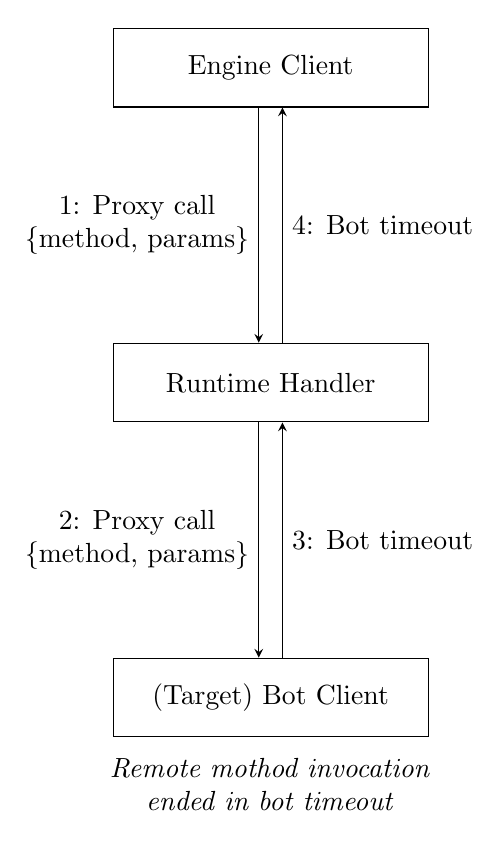
\begin{tikzpicture}[->, >=stealth, rectangle, every node/.style={minimum height=1cm, minimum width=4cm}, node distance=8cm, auto]
			
					\node [draw] (E) {Engine Client};
					\node [draw] (H) [below of = E, node distance=4cm] {Runtime Handler};
					\node [draw] (B) [below of = H, node distance=4cm] {(Target) Bot Client};

					\draw [transform canvas={xshift=-0.15cm}] (E) edge
					node[left, align=center, minimum width=0cm]
					{1: Proxy call \\ \{method, params\}} (H);
			
					\draw [transform canvas={xshift=0.15cm}] (H) edge
					node[right, align=center, minimum width=0cm]
					{4: Bot timeout} (E);
			
					\draw [transform canvas={xshift=-0.15cm}] (H) edge
					node[left, align=center, minimum width=0cm]
					{2: Proxy call \\ \{method, params\}} (B);
			
					\draw [transform canvas={xshift=0.15cm}] (B) edge
					node[right, align=center, minimum width=0cm]
					{3: Bot timeout} (H);
				
					\node [node distance=1.1cm, align=center] () [below of = B]
					{\emph{Remote mothod invocation} \\ \emph{ended in bot timeout}};
				
			\end{tikzpicture}
			\end{figure}
		\end{minipage}
		\end{adjustwidth}

%\end{document}






